\documentclass[border=2pt]{standalone}
\usepackage{tikz}
\usetikzlibrary{positioning, fit, shapes, arrows, calc}

\pgfdeclarelayer{bg}    % declare background layer
\pgfsetlayers{bg,main}  % set the order of the layers (main is the standard layer)

\newcommand{\coula}{0785F2}
\newcommand{\coulb}{F29F05}
\newcommand{\coulc}{F21313}
\newcommand{\could}{E6F21F}



\definecolor{part1}{HTML}{\coula}
\definecolor{part2}{HTML}{\coulb}
\definecolor{part3}{HTML}{\coulc}
\definecolor{part4}{HTML}{\could}

\begin{document}
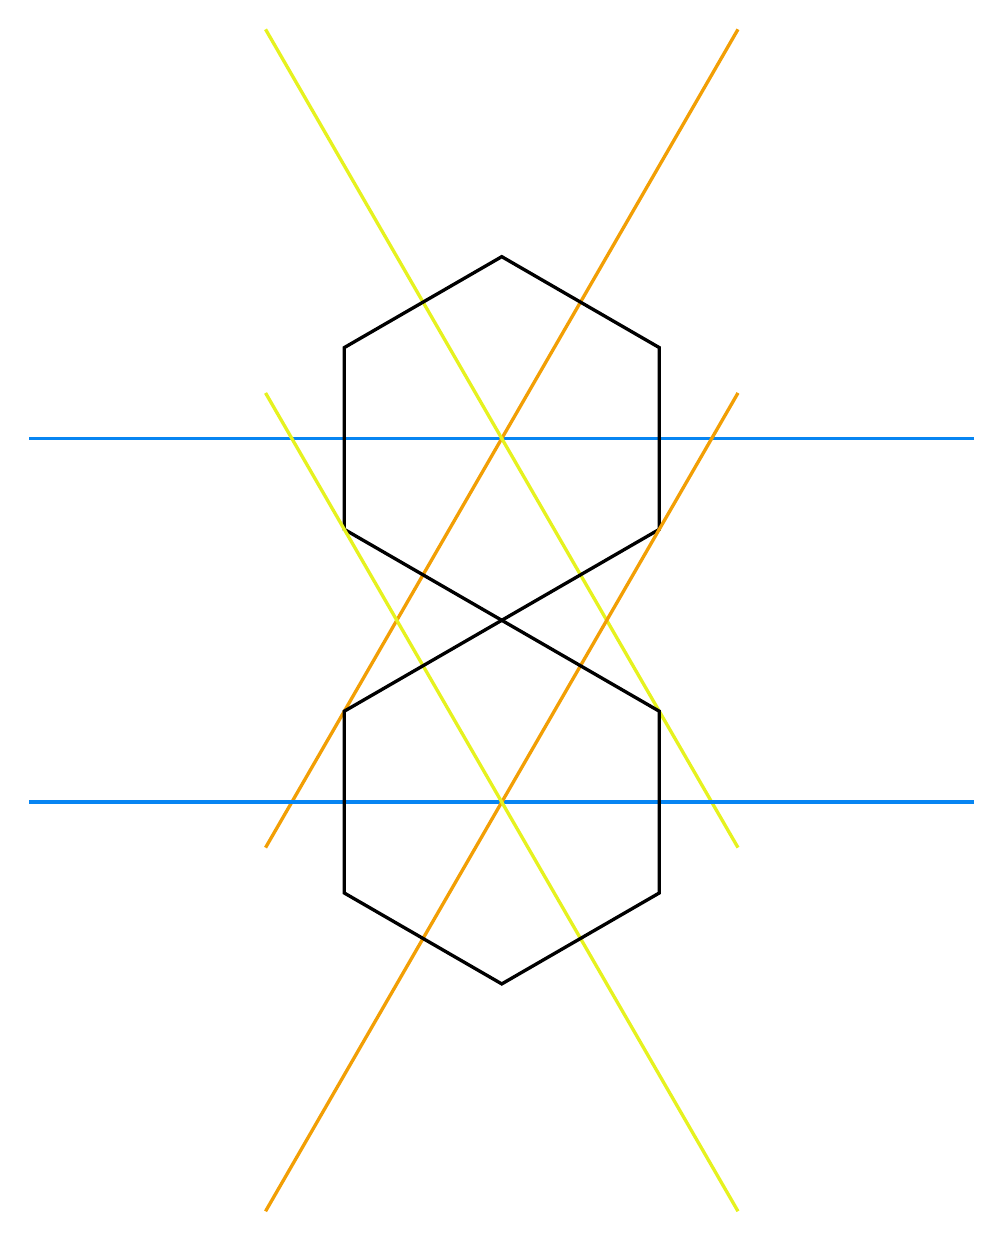
\begin{tikzpicture}[very thick]
\coordinate (A) at (0:2);
\coordinate (B) at (60:2);
\coordinate (C) at (120:2);
\coordinate (D) at (180:2);
\coordinate (E) at (-120:2);
\coordinate (F) at (-60:2);
\draw[part1]  ($3*(A)$)--($3*(D)$);
\draw[part2]  ($3*(B)$)--($3*(E)$);
\draw[part4]  ($3*(C)$)--($3*(F)$);
\draw (30:2.309)--(90:2.309)--(150:2.309)--(210:2.309)--(-90:2.309)--(-30:2.309)--cycle;
\begin{scope}[yshift = -4.618cm]
\coordinate (Ab) at (0:2);
\coordinate (Bb) at (60:2);
\coordinate (Cb) at (120:2);
\coordinate (Db) at (180:2);
\coordinate (Eb) at (-120:2);
\coordinate (Fb) at (-60:2);
\draw[part1]  ($3*(Ab)$)--($3*(Db)$);
\draw[part2]  ($3*(Bb)$)--($3*(Eb)$);
\draw[part4]  ($3*(Cb)$)--($3*(Fb)$);
\draw (30:2.309)--(90:2.309)--(150:2.309)--(210:2.309)--(-90:2.309)--(-30:2.309)--cycle;

\end{scope}

%\coordinate (Ag1) at ($(A)+(C)+(D)$);
%\coordinate (Ag2) at ($(A)+(C)$);
%\coordinate (B) at ($2*(C)+(E)$);
%\coordinate (Bg1) at ($(C)+(B)$);
%\coordinate (Bg2) at ($(C)+(B)+(E)$);
%\coordinate (G) at ($2*(F)+(D)$);
%\coordinate (Gg1) at ($(G)+(F)$);
%\coordinate (Gg2) at ($(G)+(F)+(D)$);
%\coordinate (H) at ($2*(F)+(E)$);
%\coordinate (Hg1) at ($(H)+(F)+(E)$);
%\coordinate (Hg2) at ($(H)+(F)$);
%\coordinate (F1) at ($3*(E)+2*(C)$);
%\coordinate (F2) at ($3*(E)+2*(F)$);
%\coordinate (F3) at ($3*(D)+2*(C)$);
%\coordinate (F4) at ($3*(D)+2*(F)$);
%\coordinate (123123) at ($2*(E)$);
%\coordinate (123132) at ($(C)+1.5*(E)$);
%\coordinate (123213) at ($(F)+1.5*(E)$);
%\coordinate (123231) at ($(F)+0.5*(E)$);
%\coordinate (123312) at ($(C)+0.5*(E)$);
%\coordinate (123321) at (0,0);
%\coordinate (132132) at ($(B)+(C)+0.5*(E)$);
%\coordinate (132321) at ($(C)+0.5*(D)$);
%\coordinate (132312) at ($2*(C)$);
%\coordinate (213213) at ($(H)+0.5*(E)+(F)$);
%\coordinate (213231) at ($2*(F)$);
%\coordinate (213321) at ($(F)+0.5*(D)$);
%\coordinate (231231) at ($(G)+0.5*(D)+(F)$);
%\coordinate (231321) at ($1.5*(D)+(F)$);
%\coordinate (312312) at ($(A)+(C)+0.5*(D)$);
%\coordinate (312321) at ($(C)+1.5*(D)$);
%\coordinate (321321) at ($2*(D)$);
%\draw[part1]  (Ag2)--(Gg1);
%%\draw[blue]  (Bg1)--(Hg2);
%\draw[part2]  (Bg2)--(F4);
%%\draw[red]  (F1)--(Gg2);
%%\draw[green]  (Ag1)--(F2);
%\draw[part4]  (F3)--(Hg1);
%%\draw (123123)--(123132)--(123312)--(123321)--(123231)--(123213)--cycle;
%%\draw (123132)--(123312)--(132312)--(132132)--(123132);
%%\draw (123312)--(123321)--(132321)--(132312)--cycle;
%\draw (132312)--(132321)--(312321)--(312312)--cycle;
%\draw (123213)--(213213)--(213231)--(123231)--cycle;
%\draw (123321)--(123231)--(213231)--(213321)--cycle;
%\draw (213321)--(213231)--(231231)--(231321)--cycle;
%\draw (123321)--(132321)--(312321)--(321321)--(231321)--(213321)--cycle;

\end{tikzpicture}

\end{document}
